\chapter{Apparatus}

{\color{gray}\emph{Should data results of diagnostic stuff, like Ba\textsuperscript{+} velocity (from pulses), be in this chapter?}}

This chapter describes the apparatus at Colorado State University, which we have used for all described studies of Ba/Ba\textsuperscript{+} fluorescence in SXe after deposition in vacuum.  Our main barium source, the Ba\textsuperscript{+} ion beam, is first described, as well as a purely Ba neutral source.  The co-deposit of Ba/Ba\textsuperscript{+} with Xe gas onto a cold sapphire window, subsequent laser excitation, and finally the collection optics for the fluorescence, are described.

\section{Ion Beam}

The full ion beam is shown in Fig. [ref fig ion beam w/ circuit diagram too].  {\color{red}\emph{refer to A,B etc. in figure:  }}An E$\times$B velocity filter selects Ba\textsuperscript{+}.  Pulsing plates can be used to deposit small numbers of ions with {\color{red}2-$\mu$s} pulses, which are detected with induction plates.  The main Faraday cup detects ion current from pulsing and from continuous beam mode.  Final deflection plates tune the position of deposition toward the sapphire window.

\subsection{Barium Ion Source/Acceleration}

Ba\textsuperscript{+} ions are produced in a Colutron [type?] ion gun system [reference], as depicted in Fig. x.  A solid barium charge is placed into the hollowed end of a stainless steel rod, which is then inserted into the discharge chamber, near the hot filament.  The heated barium vaporizes, and is allowed to escape the hollowed rod around a loosely threaded set screw at the end of the rod.

The source is designed to produce a discharge between the anode plate and the filament cathode, through an argon buffer(?) gas leaked into the source chamber.  This controlled discharge would then also ionize atoms from the solid charge to produce the desired ion beam.  However, to avoid contamination of our solid matrix with Ar, which could affect the spectroscopy, we do not use the buffer gas in the ion source.  As a result, {\color{red}we do not know exactly where our discharge occurs -- \textbf{don't like that}}.  It may be a between the filament and anode as designed, if a Ba pressure exists in the hot source chamber, or it may occurring elsewhere.  The longevity of our ion current from a single charge suggests that Ba is coating the inner walls of the chamber and is depleted slowly.  In any case, the discharge produces a plasma, containing barium ions, which escapes the chamber through a small hole in the anode, where it enters the acceleration potential.

The acceleration potential is 2~kV, between the ion source anode and an aperture, which constitutes \emph{THIS IS DUMB} the first element of the acceleration Einzel lens (Fig.~\ref{fig:testfig}).  This lens approximately collimates the ion beam for passage through the E$\times$B velocity filter.

\begin{figure}[H]
        \centering
                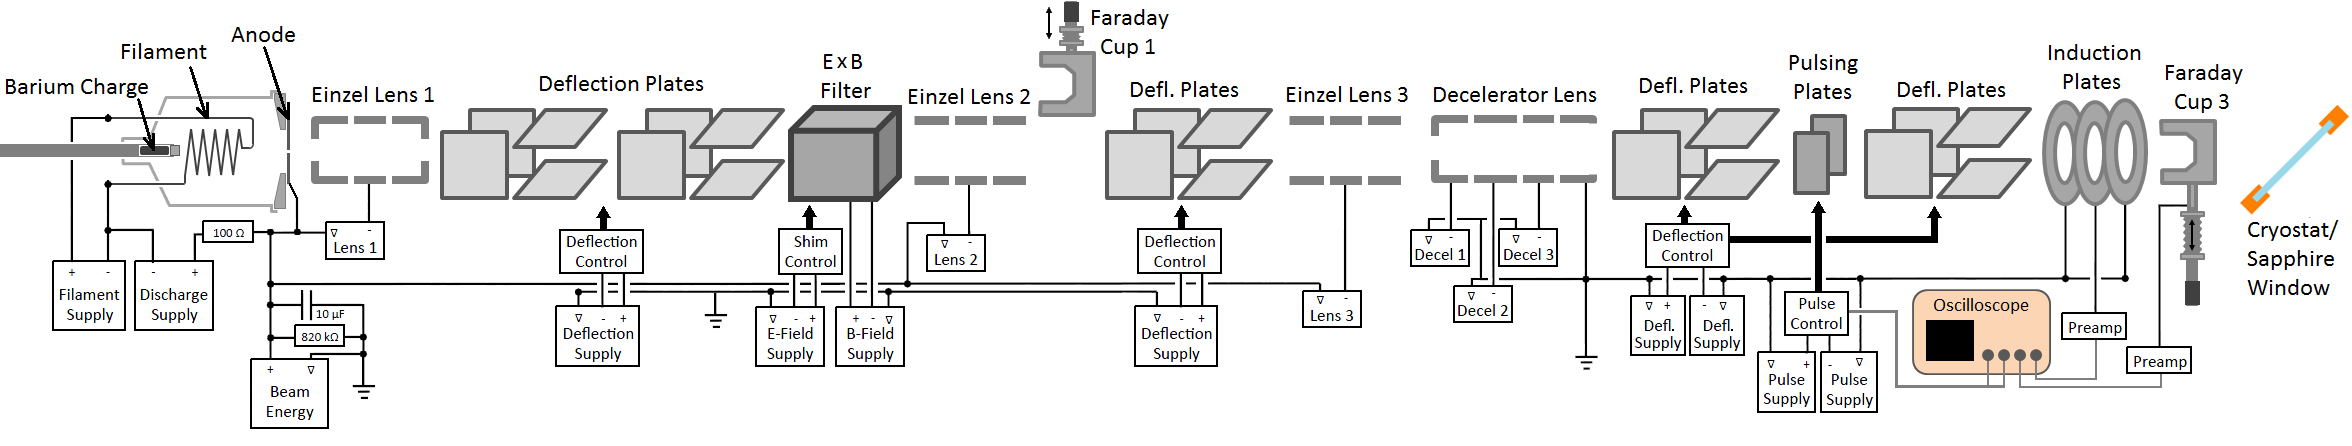
\includegraphics[width=1.\textwidth]{figures/ionBeam.png}
                \caption{ ... The decelerating lens is used only as an Einzel lens in this work, since all deposits are made at the beam's initial energy of 2~keV.  All deflection plates are set to constant values except the final set, which requires different tunings for peak ion current at Faraday cup 3 vs. the sapphire window.  {\color{red}\textbf{ExB is too bold-looking}}}
\label{fig:ionbeam}
\end{figure}

\subsection{Velocity Filter, Lensing}

The E$\times$B velocity filter selects Ba\textsuperscript{+} by creating perpendicular electric and magnetic fields, which produce opposing forces on charged particles moving straight through the filter.  Those fields are chosen such that those forces are equal for Ba\textsuperscript{+}, according to Eqn. \ref{eqn:massfilt}:

\begin{equation}
\sigma = 1.
\label{eqn:massfilt}
\end{equation}

\noindent
Other ions will be deflected, while Ba\textsuperscript{+} will continue along the beam path.

The decelerator lens has been used in the past for varying deposit energy, but it is not used in this work.  It and Einzel lens 2 are turned off.  Einzel Lens 3 focuses the beam onto the main Faraday cup (cup 3), which is used during experiments to measure ion current.  It is on a bellows for retraction during deposits.

The final set of deflection plates, H2 and V2, are also used during experiments to steer the beam for deposits.

\subsection{Ion Beam Pulsing}

When running in pulsing mode, the pulsing plates are first placed at 200~V and -200~V to deflect the beam, and are pulsed to 0~V for {\color{red}2~$\mu$s} for each pulse.  The pulsing circuit is shown in Fig. [ref fig pulsing circuit].  Square waves, triggered by LabVIEW at {\color{red}50~Hz}, enter the circuit at [x]. {\color{red}[describe how the pulse happens]}

The induction plates observe pulses during a deposit.  Pulses just prior to a deposit can be observed by cup 3 as well as the induction plates, for a local measurement of ion current in the pulses.  An example of an oscilloscope readout of {\color{red}16} averaged pulses is shown in Fig. [ref fig scope pulse -- in caption, explain v-divided plate signals].  

[x brand, or whatever] pre-amplifiers convert the ... [put this before scope picture?] [have a figure of the shaped plots too]

\subsection{Calibration of Ion Deposition}

To calibrate the signal at cup 3 to an ion density at the sapphire window, another Faraday cup (cup w) can be attached to the cold finger in place of the sapphire window.  

Firstly, the ratio in $\frac{fC}{pulse}$ between cup 3 and cup w is measured.  Then, knowing the radius of cup w lets one determine the ion density per pulse at the sapphire window:

\begin{equation}
\frac{ions}{pulse \times m^{2}} = ...
\label{eqn:ion_density}
\end{equation}

\section{Ba Getter Source}

Ba "getters" are neutral Ba sources typically used to grab reactive gas molecules in purifiers and vacuum tubes.  We can use a getter as a source of neutral Ba.

...

It is very helpful to have a completely different type of Ba source, to rule out any source-related quirks, e.g. source-produced impurities.

\section{Solid Xenon Matrix Deposition}

The final destination of the barium ions is in the solid xenon matrix, which is deposited onto a cold sapphire window.  Sapphire has good thermal conductivity, good optical transparency in the visible, and does not fluorescese in the wavelength region where barium fluoresces.  

Xenon freezes around 73~K (?) at our pressures ($0.5$ - $1 \times 10^{-7}$~Torr), so the window is cooled to temperatures below that.  The window is held to a cold finger (Fig. 6x, picture of), cooled by a -brand- cryostat. % -brand- said {\color{red}brand}, but that had errors

\subsection{Deposition Procedure}

Before barium ions are let through, xenon gas is allowed to flow, controlled by a leak valve, onto the cold sapphire window, where it freezes and begins growing the solid matrix.  The Faraday cup is then retracted, to clear the path for barium ions.  The cup serves as a shutter for DC deposition, or if pulsing is being used, they are performed at this time.  Barium ions land in the solid xenon as the matrix continues to grow.  The cup is then replaced, and the xenon leak stopped.

\subsection{Collection Optics}

talk about all that, including spectrometer